\documentclass[12pt, letterpaper]{article}
\usepackage[titletoc,title]{appendix}
\usepackage{color}
\usepackage{booktabs}
\usepackage[usenames,dvipsnames,svgnames,table]{xcolor}
\definecolor{dark-red}{rgb}{0.75,0.10,0.10} 
\usepackage[margin=1in]{geometry}
\usepackage[linkcolor=dark-red,
			colorlinks=true,
			urlcolor=blue,
			pdfstartview={XYZ null null 1.00},
			pdfpagemode=UseNone,
			citecolor={dark-red},
			pdftitle={Partisan Response}]{hyperref}

\usepackage[resetlabels,labeled]{multibib}
\newcites{SI}{SI References}
\usepackage{natbib}

\usepackage{float}

\usepackage{geometry} % see geometry.pdf on how to lay out the page. There's lots.
\geometry{letterpaper}               % This is 8.5x11 paper. Options are a4paper or a5paper or other... 
\usepackage{graphicx}                % Handles inclusion of major graphics formats and allows use of 
\usepackage{amsfonts,amssymb,amsbsy}
\usepackage{amsxtra}
\usepackage{verbatim}
\setcitestyle{round,semicolon,aysep={},yysep={;}}
\usepackage{setspace}		     % Permits line spacing control. Options are \doublespacing, \onehalfspace
\usepackage{sectsty}		     % Permits control of section header styles
\usepackage{lscape}
\usepackage{fancyhdr}		     % Permits header customization. See header section below.
\usepackage{url}                     % Correctly formats URLs with the \url{} tag
\usepackage{fullpage}		%1-inch margins
\usepackage{multirow}
\usepackage{rotating}
\setlength{\parindent}{3em}

\usepackage[T1]{fontenc}
\usepackage{bm}
\usepackage{palatino}

\usepackage{chngcntr}

\def\citeapos#1{\citeauthor{#1}'s (\citeyear{#1})}

\makeatother


% Caption
\usepackage[hang, font=small,skip=0pt, labelfont={bf}]{caption}
%\captionsetup[subtable]{font=small,skip=0pt}
\usepackage{subcaption}

% tt font issues
% \renewcommand*{\ttdefault}{qcr}
\renewcommand{\ttdefault}{pcr}

\setcounter{page}{0}

\usepackage{lscape}
\renewcommand{\textfraction}{0}
\renewcommand{\topfraction}{0.95}
\renewcommand{\bottomfraction}{0.95}
\renewcommand{\floatpagefraction}{0.40}
\setcounter{totalnumber}{5}
\makeatletter
\providecommand\phantomcaption{\caption@refstepcounter\@captype}
\makeatother

\title{Explaining Partisan Affect: Partisan Response to Partisan Response}

\author{Douglas J. Ahler\thanks{Assistant Professor of Political Science, Florida State University, \href{mailto:dahler@fsu.edu}{\texttt{dahler@fsu.edu}}} \and Carolyn E. Roush\thanks{Postdoctoral Fellow, Department of Political Science, Florida State University, \href{mailto:carolyn.roush@gmail.com}{\texttt{carolyn.roush@gmail.com}}} \and Gaurav Sood\thanks{Independent researcher, \href{gsood07@gmail.com}{\texttt{gsood07@gmail.com}}}}

\begin{document}
\maketitle
\thispagestyle{empty}

\begin{abstract}

\noindent What causes affective polarization? Past research suggests that the affective gulf between partisans is the result of greater policy disagreement or the increasing alignment of social and political identities. In this paper, we propose a third potential source of interparty animus: partisans' response to their opponents' faulty political reasoning. Specifically, we argue that partisans punish their opponents for engaging in blatant motivated reasoning but fail to hold their own side accountable for similar failures. To test this theory, we rely on two experiments deigned to exogenously manipulate perceptions of partisan motivated reasoning among partisans' co-partisans and opponents. Results from a pilot study demonstrate that Republicans appear to exhibit this ``bias blind spot,'' though the effects are imprecisely estimated; Democrats, on the other hand, did not appear engage in the same behavior. Instead, we find stronger evidence of ``partisan cheerleading'': Democrats and Republicans actually appear to \textit{punish} in-party supporters for not sufficiently engaging in biased thinking.  We discuss these results, along with a couple of anomalies, in the context of preparing for a larger-$n$, nationally representative study designed to manipulate perceptions of partisan bias in economic evalautions. We present a design that is ready to field and welcome all comments, questions, and suggestions. 

\end{abstract}

\newpage

\doublespacing
Polarization is a defining feature of contemporary U.S. politics. Increasingly, it bleeds into broader society. According to a recent Pew study, Americans perceive party conflict as the defining cleavage of the day: 86\% of Americans believe that strong conflict exists between Democrats and Republicans (with 64\% describing that conflict as ``very strong''). For comparison, 65\% of Americans say that strong conflict exists between black and white citizens, with just 27\% describing that conflict as ``very strong'' \citep{pew2018far}. At the mass level, this conflict manifests itself affectively \citep{IyengarSoodLelkes2012}. Democrats and Republicans increasingly dislike each other, see the other party as a threat to the nation's well being, discriminate against out-party supporters, and would prefer to avoid social contact with them \citep{pew_polarization}. Ultimately, some argue, this animus has the potential to undermine trust in government and democratic legitimacy \citep{hetheringtonrudolph_2015}.

What explains this increasing hostility between Democratic and Republican supporters? Obviously, there is no singular cause. We can, however, group potential explanations into broader categories. One sensible dichotomy, proposed by \citet{IyengarSoodLelkes2012}, is that partisan affect may be \emph{principled} or \emph{unprincipled}. \citeauthor{IyengarSoodLelkes2012} conceive of principled affect as grounded in policy preferences: Democrats may dislike Republicans because they find their policy positions unpalatable, and vice versa. They find little support for this hypothesis, instead arguing that ``the mere act of identifying with a political party is sufficient to trigger negative evaluations of the opposition'' (2012, 407). Subsequent research has generally supported this conclusion. For example, partisan anger and bias appear to be more related to political identities than policy preferences \citep{mason_2015}. And the psychology of affective polarization generally supports ``unprincipled animus'': not only do longstanding personality traits predict citizens' animus toward the out-party \citep{webster2018personal}, but negativity toward the other side appears to be deeply ingrained and automatic in voters' minds \citep{IyengarWestwood2014}.

But even if partisan animus doesn't stem from policy preferences \citep[e.g.,][]{rogowski2016how}---it may still be principled. People may dislike the out-party not because of what they believe, but instead because of the behavior they observe. We suspect that citizens increasingly dislike the other side because they observe their opponents engaging in blatant motivated reasoning. Examples of this type of thinking in the real world are abundant. Partisans process information in a biased way and reason toward factual conclusions that are congenial to their party, often ignoring contrary details \citep{lodgetaber_2013}. For example, who sits in the White House colors partisans' economic evaluations \citep{bartels_2002,bisgaard2015bias}, and their responses to political scandals depend on the party involved \citep{ahlersood_2014}. Moreover, these behaviors are unlikely to escape the attention of most citizens. Just as the media highlights and reinforces perceptions of social or ideological divisions among partisans, so too does it highlight and reinforce perceptions of out-party bias. For example, the kind of faulty political reasoning that often accompanies partisans' response to co-party scandals is extensively covered by the media, and particularly among outlets that do not share the partisan affiliation of those involved in the scandal \citep{budaketal_2016,puglisisnyder_2011}. 

Citizens, however, are unlikely to dwell equally on all types of partisan bias. We believe part of the reason why out-party evaluations have plummeted over time while in-party evaluations have remained relatively stable \citep{IyengarSoodLelkes2012,Hetherington2009} is because partisans tend to disproportionately attend to the bias of their opponents while ignoring their own. This phenomenon, known as the ``bias blind spot,'' is a common cognitive bias in which people can correctly identify bias in others but fail to identify errors in their own thinking \citep{proninetal_2002,pronin_2007}. In an era in which partisan identities are particularly salient \citep{bartels2000,Hetherington2001}, we suspect that this tendency extends beyond the individual to the hive mind that is the mass party --- especially because people generally ascribe good characteristics to in-groups and negative ones to out-groups in a blanket fashion \citep{alexander1999images}. And because cognitive biases are generally considered to be undesirable, observing the other side's motivated reasoning is likely to confirm partisans' preconceived notions of their opponents as ``bad people'' --- thus reinforcing attitudes and heightening affective polarization. 

In this paper, we investigate this potential source of partisan animus. To do so, we rely on two experiments to determine whether partisans' exposure to out-party bias increases their negative feelings toward other side. In this early draft, we present evidence from a pilot study suggesting that partisans' observation of out-party bias may exacerbate polarization, although these apparent effects are imprecisely estimated. Contrary to our expectations, we also find that partisans \textit{do} appear to react to bias on their own side by punishing co-partisans for not sufficiently participating in ``partisan cheerleading'' \citep{bullocketal_2015}. These findings, however, may be an artifact of flaws in our pilot design. Accordingly, we lay out our plans for administering a large-\textit{n}, nationally representative survey which we anticipate being fielded next month. %Should our theory be supported, [ADD SOME SENTENCE HERE OR SOMETHING TO CONCLUDE THIS SECTION]

\section*{Principled Partisan Affect, or a Partisan Bias Blind Spot?}

Partisans are notoriously lazy reasoners. They dismiss evidence that contradicts their own beliefs, misinterpret facts to suit their worldview, invent post-hoc rationalizations for their opinions, and generally seem unfazed by their own lousy arguments \citep{bartels_2002,druckmanetal_2013,gainesetal_2007,taber2006}. As a consequence, people mostly self-select into partisan-congenial social networks and media environments that reinforce their views \citep{stroud_2010}. When partisans do encounter their opponents' opinions, conversations are rarely productive: news feeds and comments sections across the internet are menageries of systematic inaccuracy, wishful thinking, and whataboutism (more formally defined as \emph{bolstering} by \citeauthor{abelson1959modes} \citeyear{abelson1959modes}). As a consequence, many Americans walk away from interparty conversations frustrated, angry, and feeling as if their opponents are living in a different reality. It seems quite plausible that this \emph{second-order reasoning} --- reactions to the other side's political reasoning --- could be a principled source of partisan animus. That is, partisans may dislike the other side not just because of who they are but on the validity of their opponents' reasoning. 

How principled this animus truly is, however, is another question. If partisans observe motivated reasoning on both sides of the political spectrum --- and update their feelings toward both parties accordingly --- this kind of second-order reasoning is unbiased: partisans are simply punishing faulty political reasoning regardless of its source, a behavior we could classify as \textit{principled partisanship.} This second-order reasoning could fuel dislike between the parties but would be unlikely to polarize partisan sentiments, since both Democrats and Republicans alike would ultimately become discouraged with supporters of \emph{both} parties. 

But what if people have biased second-order beliefs about partisan motivated reasoning? That is, what if partisans observe and disapprove of out-party motivated reasoning but fail to hold their co-partisans accountable for similar biases? We have good reason to suspect this might be the case. Humans are particularly adept at recognizing the impact of bias on others' judgment but regularly fail to identify how their own errors in thinking affect outcomes. The phenomenon, known as the ``bias blind spot'' \citep{proninetal_2002,pronin_2007}, is liable to exacerbate polarization. If partisans grouse about their opponents' reasoning failures while letting their co-partisans off the hook, the feelings that everyone reports about the out-party are likely to decline while in-party sentiment holds constant. This kind of \textit{motivated updating} may in fact be responsible for the pattern we've observed over the past several decades \citep{haidthetherington_2012,IyengarSoodLelkes2012} --- perhaps not coincidentally, since the emergence of ``guerilla tactics'' \citep{Schickler2001} in congressional conflict.

Another, even more perverse, possibility exists: partisans may react negatively to reasoning failures on \emph{both} sides but do so for very different reasons. That is, people might malign out-party supporters for motivated reasoning while simultaneously punishing their co-partisans for a failure to reason to the ``appropriate'' conclusion. We have reason to expect such behavior. When partisans don't know a political fact, they will often assume the party-congenial version in the absence of accuracy incentives \citep{bullocketal_2015}. This is first-order partisan cheerleading: just as Lakers fans conclude that Lonzo Ball's three-point shot will eventually fall,\footnote{The co-authors who are not rabid basketball fans have been informed that the Lakers' base is still holding out hope for Ball's redemption, despite his father's best attempts to prevent it.} Republicans believe that the FBI is ``working to delegitimize the president'' \citep{kahn2018most}. But how do citizens (or hoops fans) react when their co-partisans don't adopt those congenial conclusions? If partisans punish co-partisans for failing to reason in a motivated fashion, we would therefore observe evidence of \emph{second-order partisan cheerleading}.

We summarize these possibilities in Figure \ref{fig:typology}. The typology categorizes potential aggregate outcomes under various types of partisan reasoning. For example, if partisans observe biased reasoning among both in-party and out-party supporters and punish both parties for faulty reasoning, we find ourselves in the bottom right cell labeled \textit{principled partisanship}. As noted earlier, this type of reasoning is unlikely to yield polarization because supporters of both parties shift their opinions of the parties, in the same direction, in accordance with current events. But other forms of second-order reasoning, shown in the red cells, are more likely to polarize Democrats and Republicans. For example, if citizens only react negatively to faulty out-party reasoning --- \textit{motivated updating} --- their feelings toward the parties will polarize. On the other hand, if partisans react positively toward in-party bias, we would say they were engaging in \textit{partisan cheerleading.} In sum, if people do evaluate the parties according to the quality of their supporters' reasoning, second-order reasoning is liable to exacerbate polarization unless Democrats evaluate their co-partisans' reasoning the same way they do Republicans' (and vice versa).

\begin{figure}
\caption{A Typology of Partisan Reasoning} \label{fig:typology}
\begin{center}
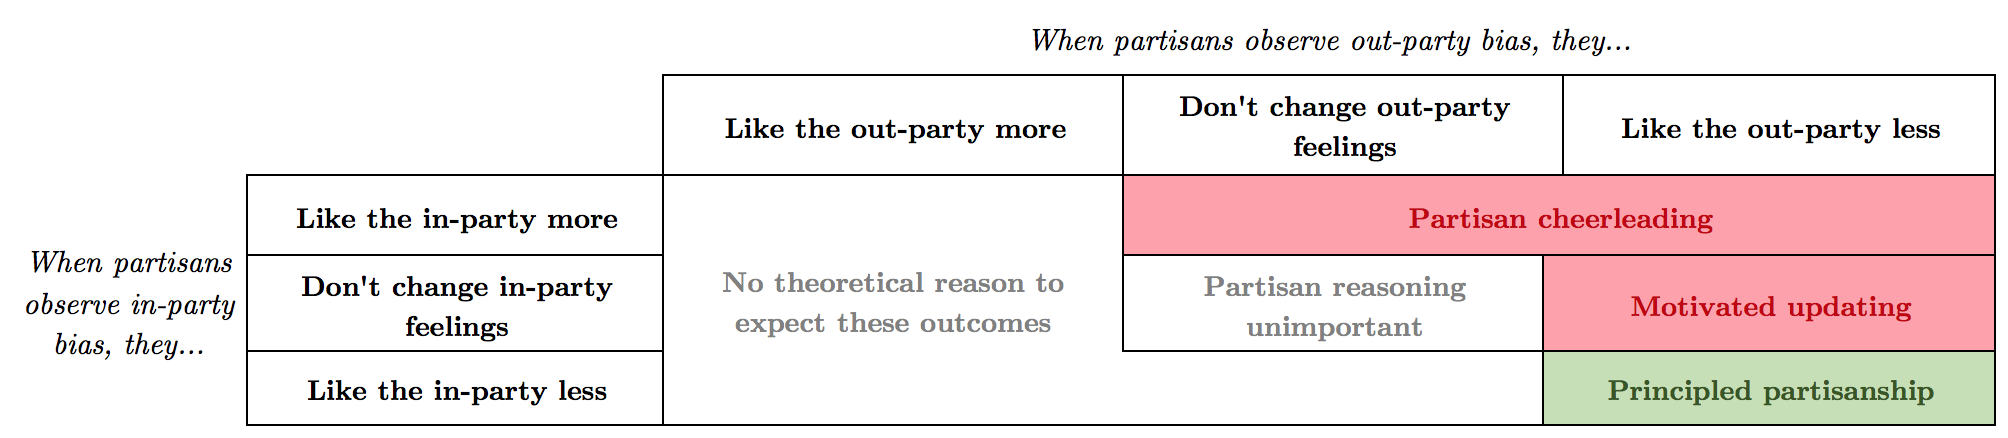
\includegraphics[scale=.48]{typology2.png}
\end{center}
\end{figure}

\section*{2013 Pilot Study: Partisan Response to Partisan Response to Controversy}

Does observation of out-party bias exacerbate affective polarization? Unfortunately, we lack the causal leverage to answer this question using observational data. Democrats and Republicans interpret real-world events through their own ``perceptual screen[s]'' \citep{campbell1960} more or less simultaneously, making it impossible to isolate any independent effect that observing out-party bias may have on out-party dislike. Furthermore, we lack real-world counterfactuals. Since partisan bias is so widespread, we rarely have opportunities observe how people react to out-partisans ``negatively updating'' their evaluations of the out-party or its leaders. To circumvent these problems, we rely upon a randomized, controlled experiment to determine if and how partisans' exposure to out-party bias exacerbates the negativity they feel for their opponents. Specifically, we use a series of vignettes featuring real political controversies and manipulate whether or not co-partisan politicians subsequently lost support among their base. This design holds constant both the controvery and the elite embroiled in the controversy, which helps to rule out important confounding variables that could muddle inferences drawn from observational data. 

We focus on controversies (and partisans' reaction to them) in this experiment for a few reasons. For one, controversies are a relatively easy way for citizens to hold politicians accountable for their actions. Typically, political accountability is assessed in one of two ways:  (1) whether elected officials espouse and pursue the policies favored by their constituents and/or (2) whether elected officials are seen as contributing positively to government performance (most commonly assessed by economic outcomes). Evaluating politicians on these bases requires a certain level of political sophistication and objectivity that most ordinary citizens lack. As a result, people often fail to hold elected officials accountable using these metrics \citep[e.g.,][]{achen2016democracy,Bartels2008,healylenz_2014,Lenz2012,snidermanstiglitz_2012,soodiyengar_2014}. Evaluating a specific controversy or misstep, on the other hand, requires much less cognitive effort and investment. For one, voters do not have to proactively search for information about these types of controversies; they are covered extensively by the media, and in particular by ideologically dissimilar outlets \citep{budaketal_2016,puglisisnyder_2011}. Secondly, controversies often surround topics that are nominally nonideological in content. For example, our vignettes feature two prominent, real world controversies concerning a salient administrative failure and a blatant attempt to prevent a high-stakes compromise. Because these outcomes are almost universally undesirable, observing the other side's failure to punish their leaders may strike partisans as particularly egregious --- thus heightening out-party animosity. 

To test this theory, we recruited 930 people to participate in a survey administered through Amazon's Mechanical Turk in November 2013. To preclude suspicion, we told respondents they would be participating in a survey on political media consumption and political learning. Prior to our experiment, we posed a question to determine whether or not respondents were paying attention to the survey. In particular, the question asked respondents to mark two particular responses. Of the 930 respondents, 38 respondents failed to complete the task as requested. We removed these participants from our sample as we felt that they were merely adding noise to the data. Because we are interested in \textit{partisans'} reactions to partisan bias, we further subset our analysis to include only self-identified and leaning partisans.\footnote{We group together ``leaning'' Independents with ``strong'' and ``weak'' partisans per previous research demonstrating Independent leaners think and behave like partisans \citep{keithetal_1992}.} Of the 726 self-identified and leaning partisans, 552 are Democrats, consistent with the general liberal bias in MTurk samples \citep{BerinskyHuberLenz2012}. 

Participants were randomly assigned to read a news story on (what was) one of three contemporary political controversies: (1) the troubled rollout of the U.S. health exchange website, Healthcare.gov (which we classify as a Democratic controversy), (2) Senator Ted Cruz's decision to force a government shutdown in order to defund Obamacare (which we classify as a Republican controversy), and (3) Toronto mayor Rob Ford's drug abuse scandal (our control). We selected these the Cruz and Healthcare.gov cases because they were timely examples of real-world, high-profile missteps that generated significant news coverage. Within these two experimental groups, we further manipulated whether Democrats' (Republicans') opinions of Obama (Cruz) changed in response to the blunder. This created five conditions based on vignette content:  (1) \textit{Democrats - Unbiased}, in which Democrats show less support for Obama post-controversy, (2) \textit{Democrats - Biased}, in which Democrats maintain high support for Obama post-controversy, (3) \textit{Republicans - Unbiased}, in which Republicans show less support for Cruz post-controversy, (4) \textit{Republicans - Biased}, in which Republicans maintain high support for Cruz post-controversy, and (5) \textit{Control.} (See Appendix A1 for vignettes.) After exposing respondents to these stories, we asked them to rate the Democratic and Republican parties using feeling thermometers. We use party feeling thermometer scores as our dependent variables in this study because they are the most common means by which to measure affective polarization \citep[e.g.,][]{haidthetherington_2012,hetheringtonrudolph_2015,IyengarSoodLelkes2012,IyengarWestwood2014,mason_2015}. 

Though our sample is disproportionately Democratic, we analyze the results of our experiment separately among Democrats and Republicans to detect any partisan differences in response to the treatments.\footnote{Research suggests that Democrats and Republicans may process information differently \citep{grossmanhopkins_2016}.} We also elect to analyze the feeling thermometers as separate dependent variables, as previous research demonstrates that the growing gulf in partisan affect has been caused primarily by increasing dislike of the out-party and not by a corresponding increase in warm in-party feelings \citep{haidthetherington_2012, IyengarSoodLelkes2012}. As out-party negativity is the ``prime mover'' over time, we might also expect our experiments to produce greater variation in the out-party feeling thermometers compared to the in-party feeling thermometers. Accordingly, our analysis produces four OLS regressions that analyze the impact of our experimental manipulation on out- and in-party affect among Democrats and Republicans. 

For each model, we include four dummy variables representing assignment to one of our experimental conditions - (1) \textit{Out-party - Unbiased} (\textit{Democrats - Unbiased} for Republicans; \textit{Republicans - Unbiased} for Democrats); (2) \textit{Out-Party - Biased} (\textit{Democrats - Biased} for Republicans; \textit{Republicans - Biased} for Democrats); (3) \textit{In-Party - Unbiased} (\textit{Democrats - Unbiased} for Democrats and \textit{Republicans - Unbiased} for Republicans); and (4) \textit{In-Party - Biased} (\textit{Democrats - Biased} for Democrats and \textit{Republicans - Biased} for Republicans).\footnote{\textit{Control} is omitted as the reference category.} Respondents receive a value of 1 if they were assigned to that particular condition and a value of 0 if they were not. The dependent variables --- the in- and out-party feeling thermometers --- range from 0 to 100. Positive coefficients indicate an increase in warmth toward the party in question; negative coefficients indicate a decrease in warmth toward the party in question.

Given our theory that partisans respond disproportionately to out-party bias and that observation of out-party bias heightens negative feelings toward the other side, we expect the largest experimental effects to appear among those respondents assigned to the \textit{Out-Party - Unbiased} or \textit{Out-Party - Biased} conditions. It is our expectation that observing the other's side lack of response to a controversy (\textit{Out-Party - Biased}) increases negative affect toward the out-party (meaning that coefficients in these conditions should be negative). Conversely, those partisans who observe the other side reacting in a more ``unbiased'' manner --- those assigned to the \textit{Out-Party - Unbiased} --- should feel, on average, more warmly toward their opponents, since the vignette suggests that their political opponents are less biased than anticipated. We have fewer expectations about how our experiment might affect people's feelings toward their own side. Since we argue partisans' response to bias is asymmetric, we do not expect information about whether one's own side engaged or did not engage in motivated reasoning to meaningfully influence in-party affect.\footnote{As noted previously, in-party feeling thermometer scores have remained relatively stable over time, which suggests these ratings are far less sensitive to stimuli than out-party ratings \citep{haidthetherington_2012, IyengarSoodLelkes2012}. The idea that in-party affect would be more difficult to move than out-party affect is also well supported by social identity research. People are motivated to maintain a positive in-group image and to disparage the out-group \citep{tajfelturner_1979}. Therefore, we might expect partisans to fail to update their evaluations of their own side when they observe in-party bias even as they more ``accurately'' update their evaluations of the other party when they observe out-party bias.} Finally, we should observe little to no effect of assignment to either the \textit{Out-Party - Unbiased} or \textit{Out-Party - Biased} conditions on \textit{in-}party affect and for a similar null effect of assignment to the \textit{In-Party - Unbiased} or \textit{In-Party - Unbiased} conditions on \textit{out-}party affect, since it is not immediately clear why information about one's own party's bias (or lack thereof) should influence feelings toward the opposite party. 

Table 1 presents the results of our experiment. We find mixed support for our hypotheses. Looking first at how our treatments may have affected Republicans' attitudes toward the Democratic Party (Column 1), we find a substantively significant increase in Republicans' warm feelings toward the Democratic Party after they were told that Democrats changed their opinions of Obama following the Healthcare.gov blunder. Republicans in this condition rated the Democratic Party on average about six percentage points warmer ($\hat{\beta}$ = 6.640) compared to those in the control group. That being said, this effect is not statistically significant at conventional levels (\textit{p}=0.22).\footnote{This is likely due to the small number of Republicans in the study.} Those Democrats who were also assigned to the \textit{Out-Party - Unbiased} condition, on the other hand, did not appear to respond significantly to the treatment. Being told that Republicans  ``correctly'' updated their approval of Cruz following the government shutdown did not appear to alter Democrats' feelings toward their opponents in any substantively or significantly meaningful way ($\hat{\beta}$ = 0.428, \textit{p}=0.89). Overall, Republicans' behavior in response to this treatment appeared to conform to our expectations while Democrats' did not.

\begin{spacing}{1}
\begin{table}[H]
\begin{center}
\captionsetup{font={it}}
\caption{Party Affect by Experimental Condition}
\bigskip
\resizebox{.8\textwidth}{!}{
\begin{tabular}{lcccc} \hline
 & \multicolumn{2}{c }{Outparty Affect} & \multicolumn{2}{c }{Inparty Affect} \\ \hline \hline
  & (1)  & (2)  &  (3) &  (4) \\
 & Republicans & Democrats & Republicans & Democrats \\ \hline
 &  &  &  &  \\
Out-Party - Unbiased & 6.640 & 0.428 & 8.991* & -6.026** \\
 & (5.409) & (2.799) & (4.943) & (2.749) \\
  &  &  &  &  \\
Out-Party - Biased & -0.972 & 1.222 & -2.880  & -2.635 \\
 & (5.409) &  (2.970) & (4.943)  & (2.918) \\
  &  &  &  &  \\
In-Party - Unbiased & 2.942 & 2.920 & -3.337  & -5.317* \\
 & (5.190) & (2.848) & (4.744) & (2.798) \\
  &  &  &  &  \\
In-Party - Biased & -4.191 &  4.075 & 1.375  & -1.102 \\
 & (5.314) & (2.820) & (4.859)  & (2.270) \\
  &  &  &  &  \\
Constant & 30.585*** &  23.580*** & 63.171*** & 68.010*** \\
 & (3.549) & (2.078) & (3.244)  & (2.042) \\
 &  &  &  &  \\
Observations & 172 & 552 & 172  & 552 \\
 R-squared & 0.025 & 0.006 & 0.042 & 0.013 \\ \hline
&  &  &  &  \\
\multicolumn{5}{c}{ Standard errors in parentheses.} \\
\multicolumn{5}{c}{ ***\textit{p}$<$0.01, **\textit{p}$<$0.05, *\textit{p}$<$0.1, two-tailed.} \\
\end{tabular}}
\bigskip
\captionsetup{font={footnotesize,it}}
\caption*{Source: 2013 MTurk Study.}
\end{center}
\end{table}
\end{spacing}

\bigskip
Assignment to the \textit{Out-Party - Biased} condition, on the other hand, did not appear to alter either Democrats' or Republicans' feelings toward their opponents (Columns 1 and 2). Neither coefficient ($\hat{\beta}$ = -0.972, \textit{p}=0.86 for Republicans; $\hat{\beta}$ = 1.222, \textit{p}=0.68 for Democrats) is substantively or statistically significant. While our original expectation was that assignment to these conditions would moderate out-party antipathy, we instead find that informing partisans that the other side maintained its support for their leader in the wake of controversy has little to no substantive effect on their out-party evaluations. 

While these results may appear puzzling at first, our treatments may have failed to move out-party affect because partisans are predisposed to assume that the out-party will react in a biased manner. That is, partisans may anticipate that out-party politicians will continue to receive sustained support from their followers after a scandal because such behavior is commonplace in American politics.\footnote{Indeed, previous work demonstrates that co-party politicians do not tend to lose support among partisans in the wake of scandals \citep{ahlersood_2014,stoker_1993}.} This may also explain why we see more of an effect (at least among Republicans) in the \textit{Out-Party - Unbiased} condition: respondents were affected more by news that the out-party was \textit{unbiased} because this information is unusual and surprising \citep[e.g.,][]{maheswaranchaiken_2011}.

Some of the largest experimental effects emerge in those conditions in which we expected null results. Perhaps most interestingly, both groups of partisans appeared to feel \textit{less} warmly toward their own side after being told co-partisan politicians lost support among their base (row 3 in Columns 3 and 4). On average, those Republicans who were told that Cruz's approval dropped rated the Republican Party three percentage points more negatively (though this effect is not statistically significant at conventional levels; $\hat{\beta}$ = -3.337, \textit{p}=0.48). The effect among Democratic respondents in the \textit{In-Party - Unbiased} condition was also substantively large and statistically significant; on average, those Democrats who were told their copartisans approved less of Obama following the misstep rated their own party about five degrees cooler ($\hat{\beta}$ = -5.317, \textit{p}=0.06). Taken together, these results suggest that while partisans may punish the other side for engaging in motivated reasoning, they actually \textit{reward} their own side for exhibiting favorable bias toward a co-party politician. In this way, partisans seem to approve of ``partisan cheerleading'' \citep{bullocketal_2015} on their own side but punish their opponents for engaging in the same practice. 

Finally, we find some unexpected and perplexing results in our remaining conditions. Specifically, we find that out-party affect appears to be responsive to cues from one's own party and vice versa. While most of these effects are not statistically significant, their direction and magnitude warrant a closer look. For example, both Republicans and Democrats who were told that their own party reneged its support for a co-partisan leader rated the \textit{other party}, on average, about three degrees warmer than their co-partisans in the control group ($\hat{\beta}$ $_{\textit{In-Party - Unbiased}}$ = 2.942, \textit{p}=0.57 for Republicans; $\hat{\beta}$ $_{\textit{In-Party - Unbiased}}$ = 2.920, \textit{p}=0.30 for Democrats). We also found that both groups of partisans appeared to rate their own side about three degrees \textit{cooler} after learning that the other side engaged in motivated reasoning ($\hat{\beta}$ $_{\textit{Out-Party - Biased}}$ = -2.880, \textit{p}=0.56 for Republicans; $\hat{\beta}$ $_{\textit{Out-Party - Biased}}$ = -2.635, \textit{p}=0.36 for Democrats). 

For the remaining conditions, we found that Democrats and Republicans differed in their responses to the same treatment. For example, those Republicans who were told that their own party engaged in motivated reasoning (\textit{In-Party - Biased}) rated the other side about four percentage points \textit{less} favorably ($\hat{\beta}$ = -4.191, \textit{p}=0.43), while Democrats responded by rating the other side about four percentage points \textit{more} favorably ($\hat{\beta}$ = 4.075, \textit{p}=0.15). While neither of these effects are statistically significant, we find a similar discrepancy in partisans' response to the \textit{Out-Party - Biased} condition. Here, we find that Republicans rated their own party a statistically significant nine percentage points warmer when they observed a loss in Democratic support for Obama ($\hat{\beta}$ = 8.991, \textit{p}=0.07), and Democrats rated their own party a statistically significant six points cooler after observing similar behavior among Republicans ($\hat{\beta}$ = -6.026, \textit{p}=0.03). These are, in fact, the largest effect sizes in the study and among the few that are statistically significant at conventional levels. While the discrepancy between positive and negative effects may be reflective of the fact that partisans think differently from one another \citep{grossmanhopkins_2016}, we are nevertheless puzzled by the fact that out- (in)-party feeling thermometers move significantly in response to in- (out)-party treatments. We welcome any and all thoughts or interpretations concerning these results. 

\section*{Research Design, Study II: Partisan Response to Partisan Retrospective Evaluations}

While some of the results above conformed to our expectations, many others did not. There are, however, some flaws in the study's design that suggest it may not be the best test of our theory. First, the relatively small number of respondents in the study makes it difficult to draw reliable statistical inferences. This is particularly problematic when drawing generalizations about Republican identifiers; on average, each experimental group had only a little more than 30 Republican respondents. While there are fewer statistical obstacles to analyzing Democrats' behavior in the study --- each condition had about 100 Democratic respondents --- we may still lack a large enough sample size to detect small effects \citep[e.g.,][]{cohen_1992}. 

Secondly, our treatments may not be strong enough to move partisan affect. In the design above, we manipulated perceptions of motivated reasoning by exposing participants to partisans' biased/unbiased approval ratings of political leaders. While bias in approval ratings is certainly one manifestation of motivated reasoning, it is also one of the most commonly observed in American politics. People may anticipate --- and accept --- that partisans will always favor in-party politicians and dislike out-party politicians because approval ratings are consistently tightly correlated with party identification.\footnote{This might also explain why we observe partisans punishing their own side for not engaging in bias in our pilot study: they see approval ratings as a mostly partisan attitude and dislike it when their co-partisans fail to sufficiently support their ``team.''} Other types of motivated reasoning would perhaps strike partisans as less benign. For example, partisans overly incorporate congenial information and dismiss evidence that challenges their beliefs, even when arguments against their position are much stronger than their own side's \citep{druckmanetal_2013,taber2006}. Furthermore, they frequently misinterpret objective facts in order to maintain consistency with their prior beliefs \citep{bartels_2002,gainesetal_2007}. Partisans may, in fact, increase their negative perceptions of the other side after being made aware of more brazen instances of motivated reasoning. 

Finally, our design in the pilot does not test how partisans might respond when they are exposed to information demonstrating \textit{both} in- and out-party bias. That is, we only tested how partisans responded to evidence of bias (or lack thereof) from one party at a time. In the real world, however, partisans often observe simultaneous partisan bias from both sides in reacting to the same news, fact, or event. Does being made aware of one's own biases attenuate the hostility partisans may feel when observing the other side engaging in motivated reasoning? While we think this is unlikely to be the case, we have not yet explored this possibility. 

In an attempt to improve upon these flaws, we plan on administering a new survey to a nationally representative sample of adults in April 2018. Working with YouGov, we will recruit 1,500 participants --- including equal numbers of Democrats and Republicans\footnote{A larger \textit{n} and a balance on party identification will allow us to circumvent the small sample problems we encountered in the pilot study.}  --- to participate in an experiment that we believe provides a clearer test of our theory.\footnote{We had originally prepared to administer this as part of an omnibus, cross-institutional survey in early March 2018, but circumstances beyond our control forced us to delay its launch. Instead, we present our research design here, and welcome any suggestions or critiques that might improve the experiment.} Once again, to preclude suspicion, we will tell respondents that they will be participating in a survey designed to understand how people learn and what they pick up from various media. 

We plan to manipulate perceptions of motivated reasoning by selectively exposing respondents to information about real-world changes in partisans' economic evaluations following the election of Donald Trump. Gallup polls administered just a week before and a week after the 2016 election demonstrated that partisans significantly shifted their evaluations of the economy in response to Trump's victory: namely, Republicans became more optimistic while Democrats became more pessimistic.\footnote{Specifically, prior to the election, only 16\% of Republicans believed the economy was getting better, compared to 49\% just a week later. At the same time, the percentage of Democrats who said the economy was improving dropped from 61\% to 46\% \citep{gallup_econ}.} This kind of bias, we believe, will strike partisans as more egregious than that inherent in approval ratings. Partisans may tolerate bias in approval ratings because they constitute a subjective partisan \textit{attitude}; tolerating bias in the interpretation of political \textit{facts}, on the other hand, is an entirely different matter. We believe observing this kind of bias might inspire more pronounced changes in partisan affect. 

To construct our treatments, we altered an article from \textit{Business Insider} that highlighted these phenomena. Specifically, we changed the original title --- ``Republicans and Democrats Have Dramatically Shifted Their Views of the U.S. Economy Since the Election'' \citep{bi_2016} --- and content of the article to fit one of three treatment conditions: (1) one that highlights the Democrats' shift (``Democrats Have Dramatically Shifted Their Views...'' - \textit{Democrats - Biased} condition), (2) one that highlights the Republicans' shift (``Republicans Have Dramatically Shifted Their Views..." - \textit{Republicans - Biased} condition), and (3) one that highlights the shifts among both partisan groups (preserving the original headline - \textit{Bipartisan Bias} condition). In addition to altering the title and portions of the text, we also made two more modifications to the original article in constructing our treatments. First, we added a quote from an out-party supporter reacting to the shift, per previous research suggesting that narratives are more persuasive than statistics \citep{Kahneman2011}.\footnote{For the third treatment condition displaying bipartisan bias, we included quotes from in-party and out-party members.} Second, we added a graph showing displaying the trends described in the article to reflect the fact that the addition of images and/or illustrations increases reading comprehension \citep{gambrelljawitz_1993}. 

In addition to our three treatment conditions, we also created a control condition using a slightly modified version of an article from \textit{The Hill} concerning the results of a recent poll about the economy.\footnote{Once again, we added a graph that summarizes the text of the article to maintain as much visual similarity as possible in the vignettes across conditions.} This piece only reports the aggregate results from the poll; it does not highlight any differences in evaluations across partisan groups. We believe that by holding the subject matter --- economic evaluations --- across treatment and control groups, we can isolate the effect of exposure to biased partisan perceptions while ameliorating any concerns related to differences in topic selection. (See Appendix A2 for experimental vignettes.) 

Following random assignment to one of these four groups, respondents will once rate the parties using the party feeling thermometers. As was the case in our previous experiment, we expect partisans to disproportionately punish theiropponents for engaging in bias while either failing to punish or rewarding their own side for exhibiting the same kind of faulty reasoning. That is, we should observe those partisans who observe out-party bias (Democrats in the \textit{Republicans - Biased} condition and Republicans in \textit{Democrats - Biased} condition) to exhibit more negative out-party feelings than their counterparts in the control group. On the other hand, we expect that partisans who observe bias on their own side (Democrats in the \textit{Democrats - Biased} condition and Republicans in \textit{Republicans - Biased} condition) will differ little from their counterparts in the control group when it comes to the average score they assign to their own party. While we observed some evidence of partisan cheerleading in our earlier experiment --- that is, partisans appeared to feel more negatively toward their own side after being told that their fellow partisans did \textit{not} engage in bias --- we do not necessarily expect similar results in this experiment. Whereas people may want their co-partisans to maintain support for an embroiled co-party politician, it is less likely that they will be disappointed in their co-partisans for not engaging in more blatant partisan reasoning. While we do not necessarily expect partisans to punish their own side for exhibiting bias, we do expect them to largely overlook in-party bias and disproportionately focus on the biased reasoning of the out-party \citep{proninetal_2002,pronin_2007}. For similar reasons, we also expect an asymmetric partisan response among respondents assigned to the \textit{Bipartisan Bias} condition. Even though respondents in this condition will be made aware of their own side's biases, we do not expect them to temper their evaluations of the out-party accordingly. Therefore, we should expect those assigned to the \textit{Bipartisan Bias} to behave similarly to those assigned to conditions highlighting in- or out-party bias: partisans should not meaningfully change their evaluations of their own side, but should continue to reward the faulty reasoning of the out-party with more negative feeling thermometer scores. 

Finally, we also plan to ask respondents to rate how well a series of personality traits --- including ``ignorant,'' ``sincere,'' ``open to reason,'' ``smug,'' ``selfish,' ``patriotic,'' and ``hypocritical''\footnote{These trait evaluations regularly appear in large scale surveys like the American National Election Studies.} --- describe Democrats and Republicans. The benefit here is twofold. First, partisans' divergence in trait ratings is indicative of affective polarization \citep{hetheringtonlongrudolph_2016}. Asking respondents to make these evaluations post-treatment thus gives us another set of dependent variables to analyze for evidence that our experiment produced changes partisan affect. Secondly, examining whether differences emerge across treatment groups for the ``hypocritical'' or ``open to reason'' ratings in particular might help us pinpoint the specific mechanism linking bias to party animus. While we do not specifically prime specific traits in our vignettes, we believe that these terms (or concepts) in particular are activated when partisans observe out-party bias. Seeing evidence of the out-party's flawed thinking may cause partisans to conclude that their opponents are impervious to facts. Therefore, we should expect those partisans who observe out-party bias to characterize the opposition as less ``open to reason'' than their counterparts in the control group. Similarly, observing evidence of out-party bias may prompt respondents to see the other side as ``hypocritical,'' as it can be used as ammunition to explain away prior accusations of bias from the out-party.\footnote{Admittedly, our thinking here is underdeveloped. But we do have a strong suspicion that observing instances of hypocrisy and ``whataboutism'' are tightly connected to negative out-party affect.} Accordingly, we should expect partisans exposed to out-party bias to rate the other party as more hypocritical than their counterparts in the control group. Of course, given the theory we laid out above, we should again observe an asymmetry in response: those partisans who observe bias on the part of their own party --- even in the \textit{Bipartisan Bias} condition --- should not be any more likely to ascribe these negative traits to their own side. 

\section*{Discussion and Conclusion}

When partisans debate each other, scroll through Facebook, watch certain cable news programs, or read comments sections online, they are likely to encounter motivated reasoning``on both sides.'' How they react has implications for affective polarization. If citizens hold their opponents accountable for their faulty reasoning while excusing their own, their out-party disdain would grow while their in-party sentiments would hold steady --- exactly the pattern we've observed over past decades \citep{IyengarSoodLelkes2012}. 

How do citizens reason about partisan motivated reasoning? The data from our pilot study are largely inconclusive but suggest interesting patterns. Republicans' feelings toward Democrats improve six points when told that Democrats \emph{did not} reach motivated conclusions when thinking about the bungled Healthcare.gov rollout, but with so few Republican respondents, this apparent effect is imprecisely estimated. Democrats, on the other hand, did not appear fazed by information that Republicans punished Ted Cruz for his \emph{Green Eggs and Ham} stunt, but neither did they react to information that Republicans did not do so. More apparent is evidence of second-order partisan cheerleading: supporters of both parties appear to rate their co-partisans more negatively upon learning they reacted to an in-party controversy in an \emph{unbiased} manner.\footnote{Pooling across Democratic and Republican respondents, $\hat{\beta}=-3.3$ feeling thermometer points, $(p=0.08)$} In sum, the evidence thus far suggests that when party supporters observe faulty partisan reasoning, they are liable to end up in the upper right cell in Figure \ref{fig:typology}: party cheerleading, coupled with the possibility of motivated updating, which can polarize partisan sentiment.

This comes with a huge caveat. Not only are these results imprecisely estimated and relatively opaque, but theory-unexpected results further muddle interpretation. Among the largest apparent effects from the pilot: Republicans' feelings toward their own party improve when they learn that Democrats punish Barack Obama for Healthcare.gov's initial failure, while Democrats' feelings toward their own party worsen when they learn Republicans punish Ted Cruz for his role in the shutdown. It is possible these discrepant results stem from differences between the two treatments. It is also possible the sample plays a role: MTurk Republicans tend to be outside the party mainstream. For these reasons, we are planning a nationally-representative survey with treatments that are as identical as possible across respondent partisanship. Furthermore, we propose presenting respondents with evidence of partisan motivated reasoning (or not) about economic facts, which may seem more egregious --- and thus provide higher-impact, clearer treatments.

We suspect that partisan animosity has many roots. The existing dichotomy between ``principled'' and ``unprincipled'' sources of affective polarization overlooks a third possibility: partisans may have a principled basis for disliking the other party, but fail to recognize that same behavior among their own side. We find this a fruitful avenue of research, in part because it may provide a relatively easy cure for polarization. People may be bad at reasoning, but even \citet{Kahneman2011} argues they can learn to recognize their cognitive biases. We can't change people's identities --- the primary unprincipled source of polarization --- and to the degree that citizens have independent policy preferences, we would not deign to change such a principled basis. A principled-but-flawed basis, if it exists, seems an appropriate target. We welcome any comments, questions, and suggestions at this early stage.

\clearpage

\bibliographystyle{apsr}
\bibliography{xperceive}

\clearpage

\appendix
\renewcommand{\thesection}{A \arabic{section}}
\renewcommand\thetable{\thesection.\arabic{table}}  
\renewcommand\thefigure{\thesection.\arabic{figure}}
\counterwithin{figure}{section}

\begin{center}
\Large{Appendix}
\end{center}

\section{Pilot Experimental Vignettes}

\begin{figure}[ht]
\centering
\begin{minipage}[b][12cm][b]{0.45\linewidth}
\caption{Democrats - Unbiased}
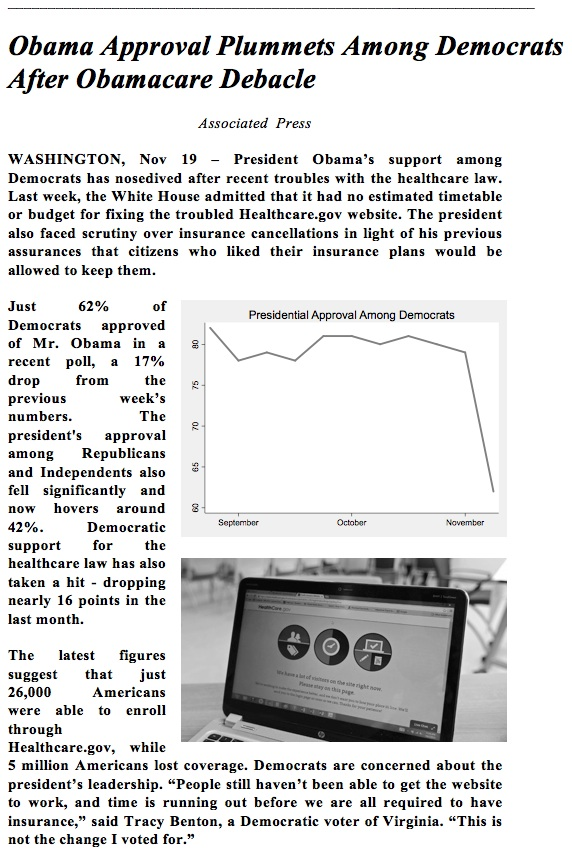
\includegraphics[width=1.05\textwidth]{Dem_C.jpg}
\label{fig:minipage1}
\end{minipage}
\quad
\begin{minipage}[b]{0.45\linewidth}
\caption{Democrats - Biased}
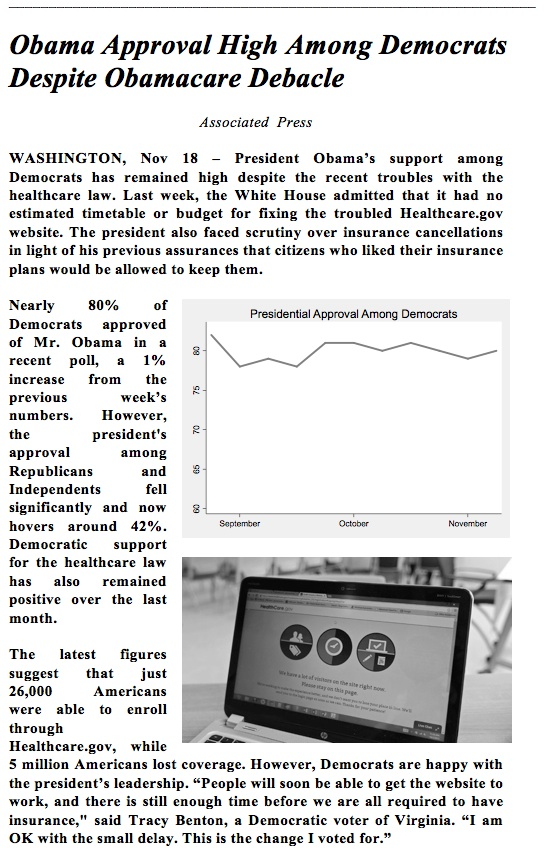
\includegraphics[width=1\textwidth]{Dem_T.jpg}
\label{fig:minipage2}
\end{minipage}
\end{figure}

\begin{figure}[ht]
\centering
\begin{minipage}[b][12cm][b]{0.45\linewidth}
\caption{Republicans - Unbiased}
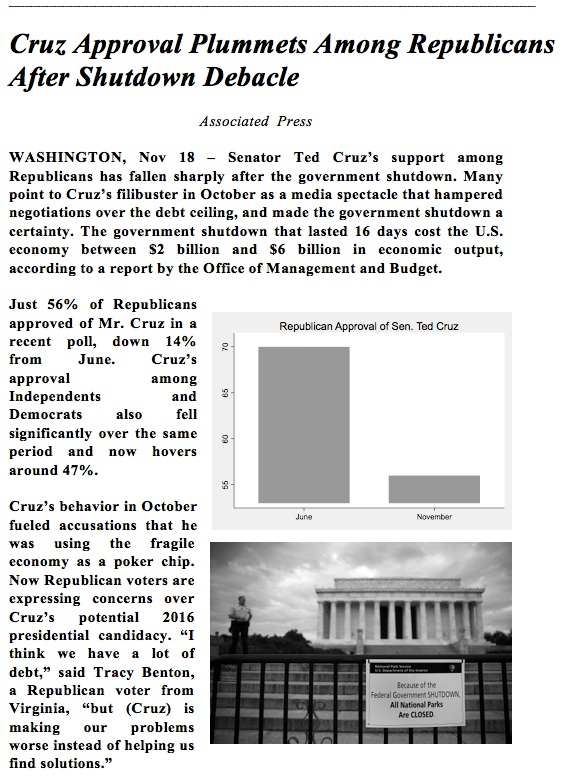
\includegraphics[width=1.05\textwidth]{Rep_C.jpg}
\label{fig:minipage3}
\end{minipage}
\quad
\begin{minipage}[b]{0.45\linewidth}
\caption{Republicans - Biased}
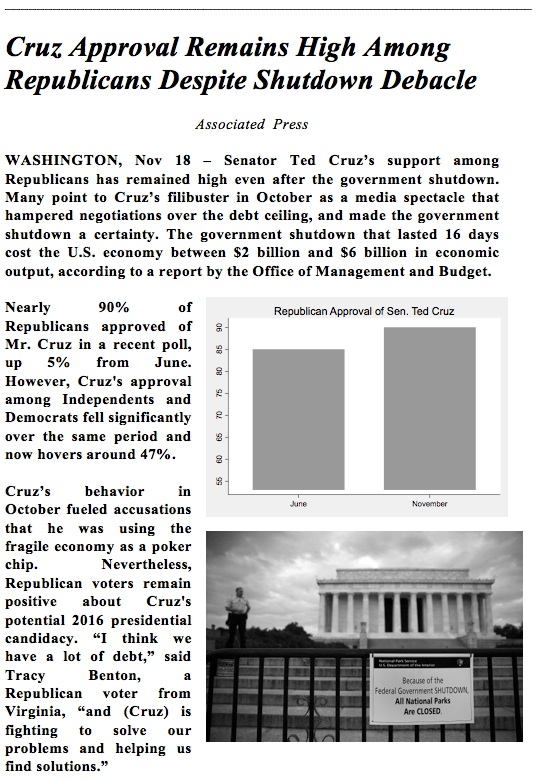
\includegraphics[width=1\textwidth]{Rep_T.jpg}
\label{fig:minipage4}
\end{minipage}
\end{figure}

\begin{figure}[ht]
\centering
\begin{minipage}[b][12cm][b]{0.45\linewidth}
\caption{Control}
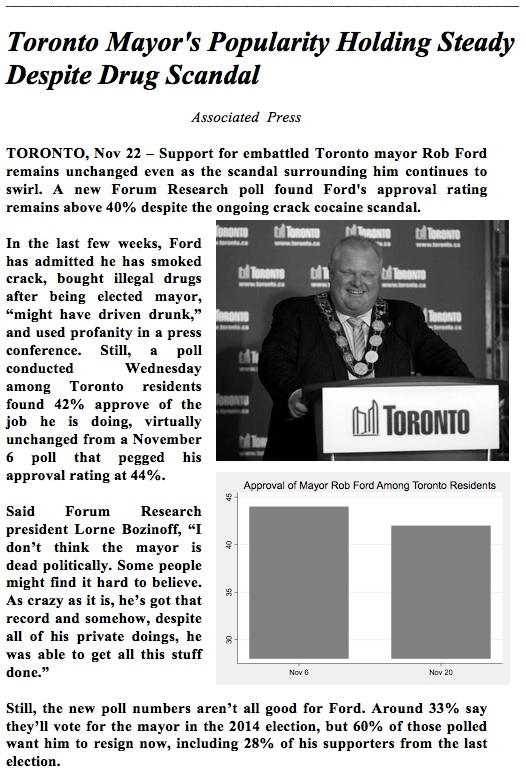
\includegraphics[width=1.05\textwidth]{P.jpg}
\label{fig:minipage5}
\end{minipage}
\end{figure}
\clearpage

\section{Study II Experimental Vignettes}

\begin{figure}[H]
\centering
\captionsetup{font={it}}
\caption{Republican Bias}
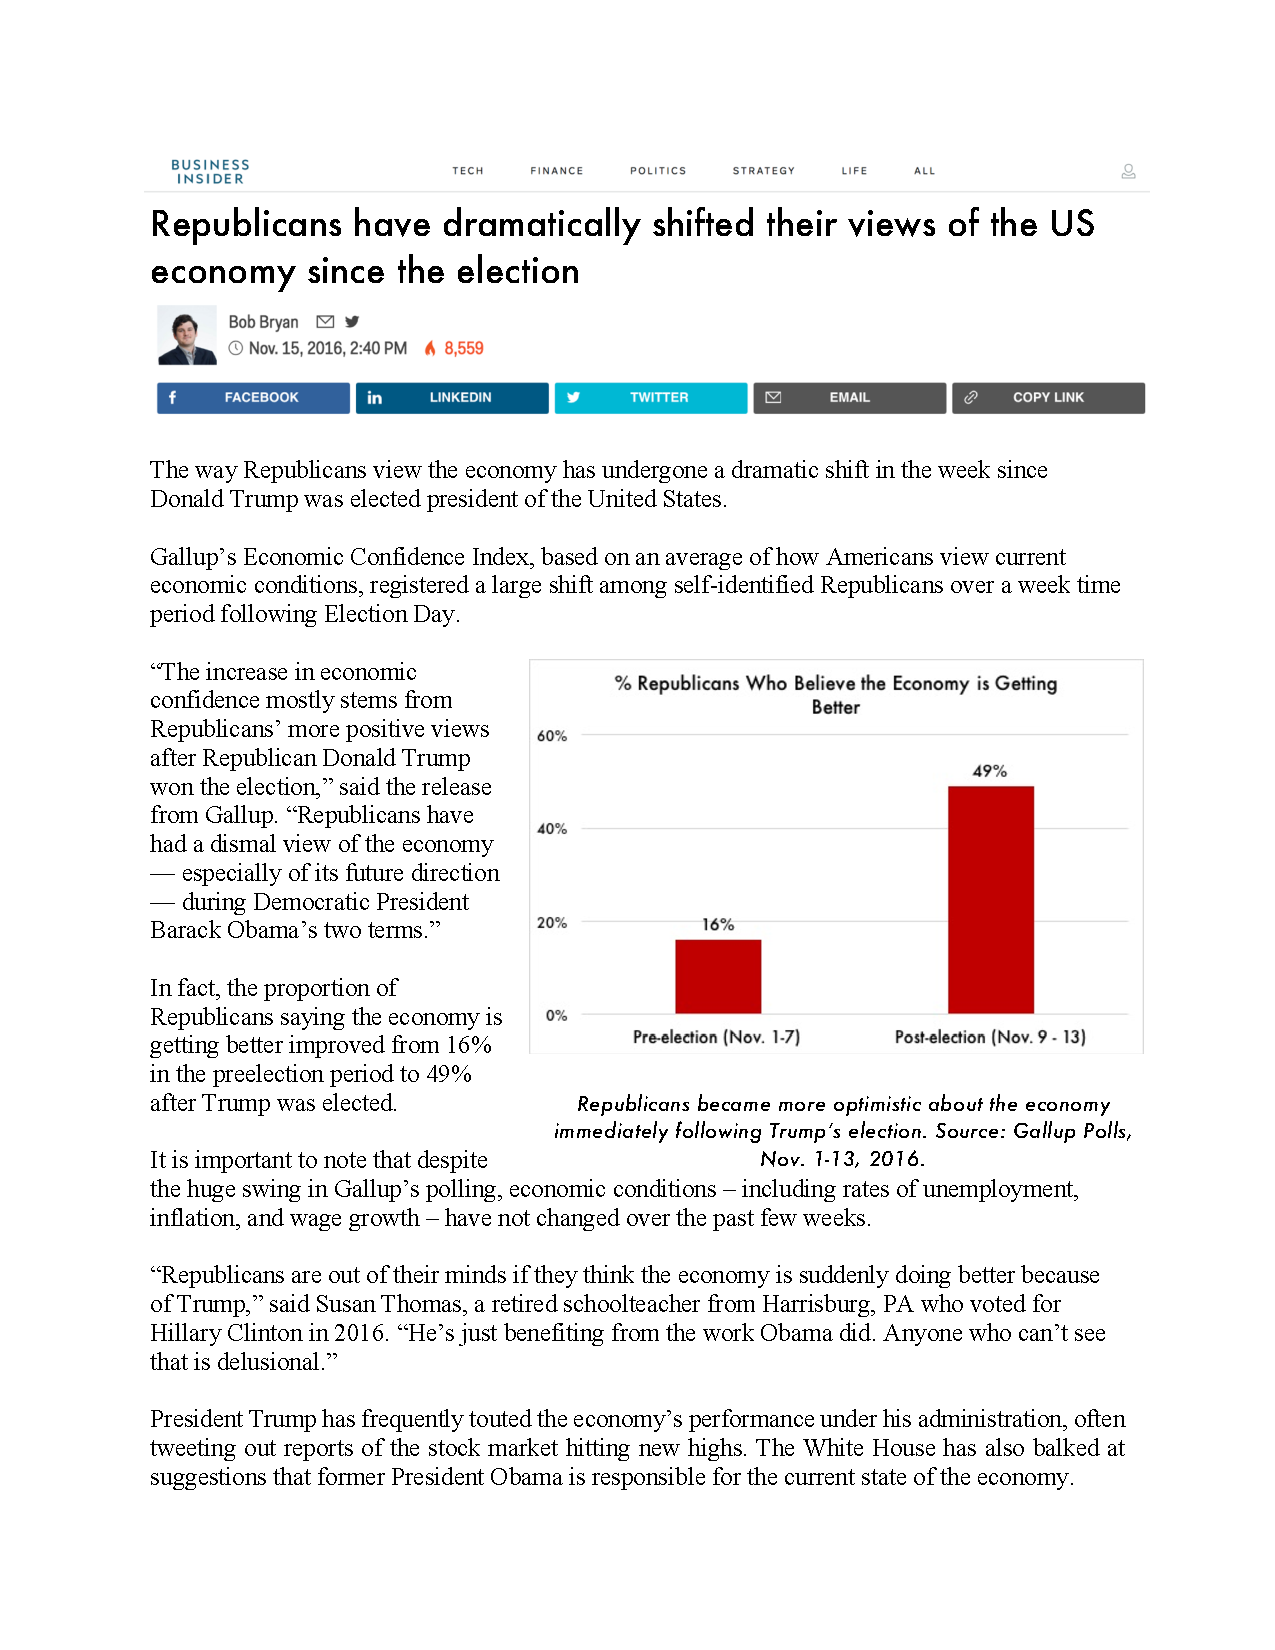
\includegraphics[width=1.05\textwidth]{rep_motivate.pdf}
\smallskip
\end{figure}

\begin{figure}[H]
\centering
\captionsetup{font={it}}
\caption{Democratic Bias}
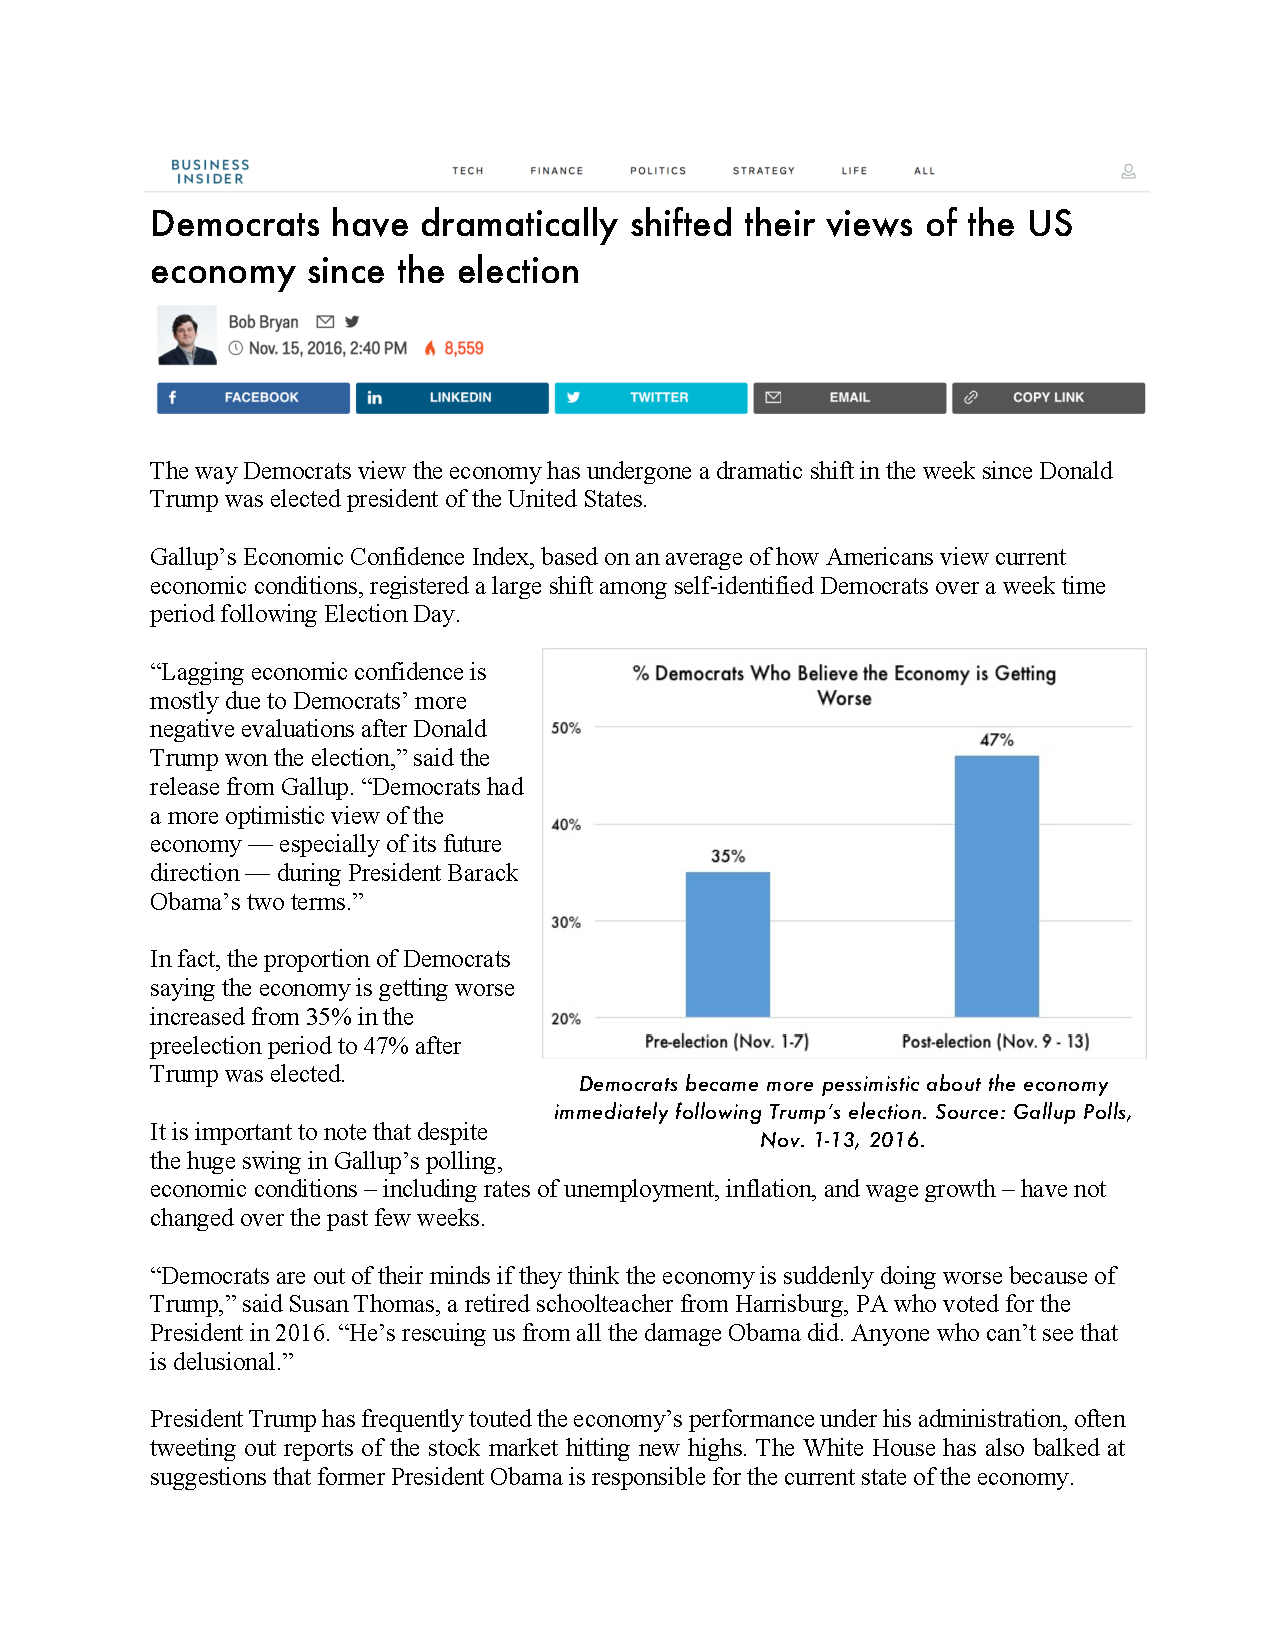
\includegraphics[width=1.05\textwidth]{dem_motivate.pdf}
\smallskip
\end{figure}

\begin{figure}[H]
\centering
\captionsetup{font={it}}
\caption{Bipartisan Bias}
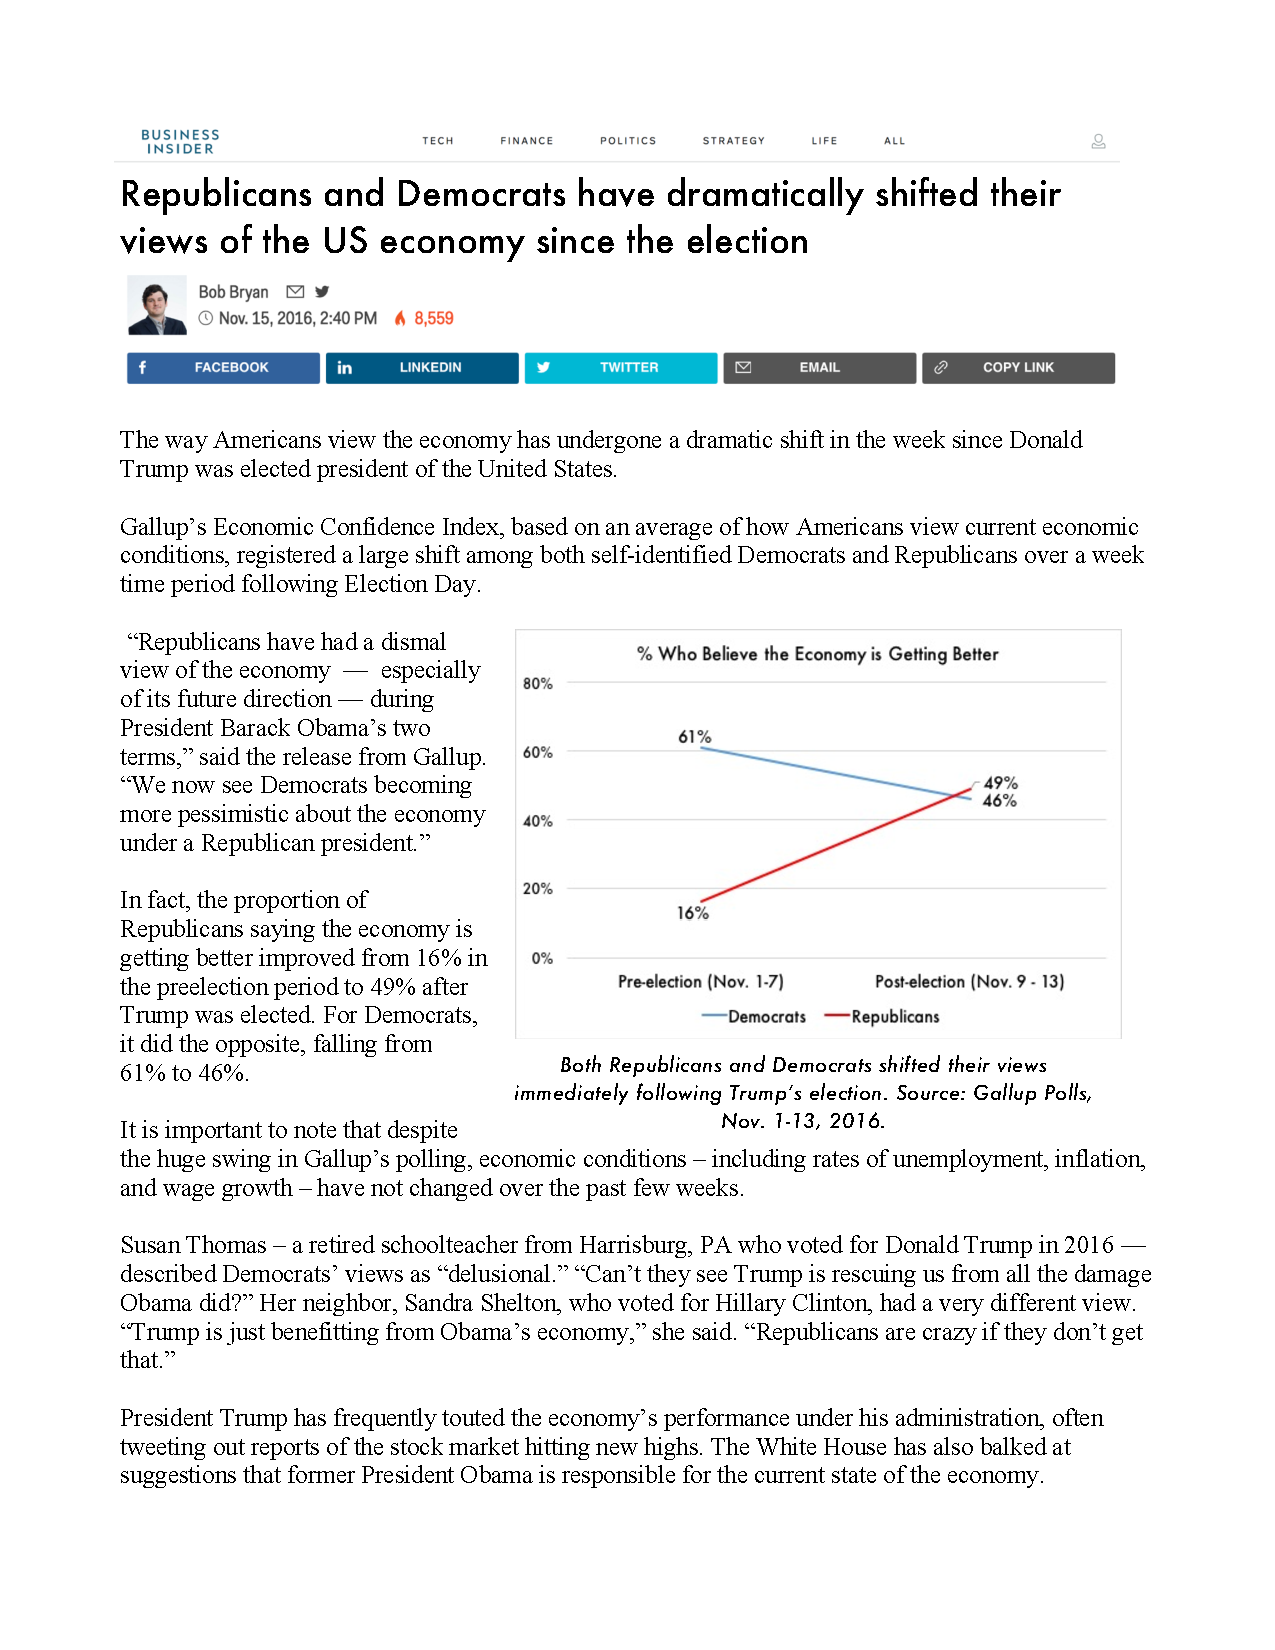
\includegraphics[width=1.05\textwidth]{bipart_motivate.pdf}
\smallskip
\end{figure}

\begin{figure}[H]
\centering
\captionsetup{font={it}}
\caption{Control}
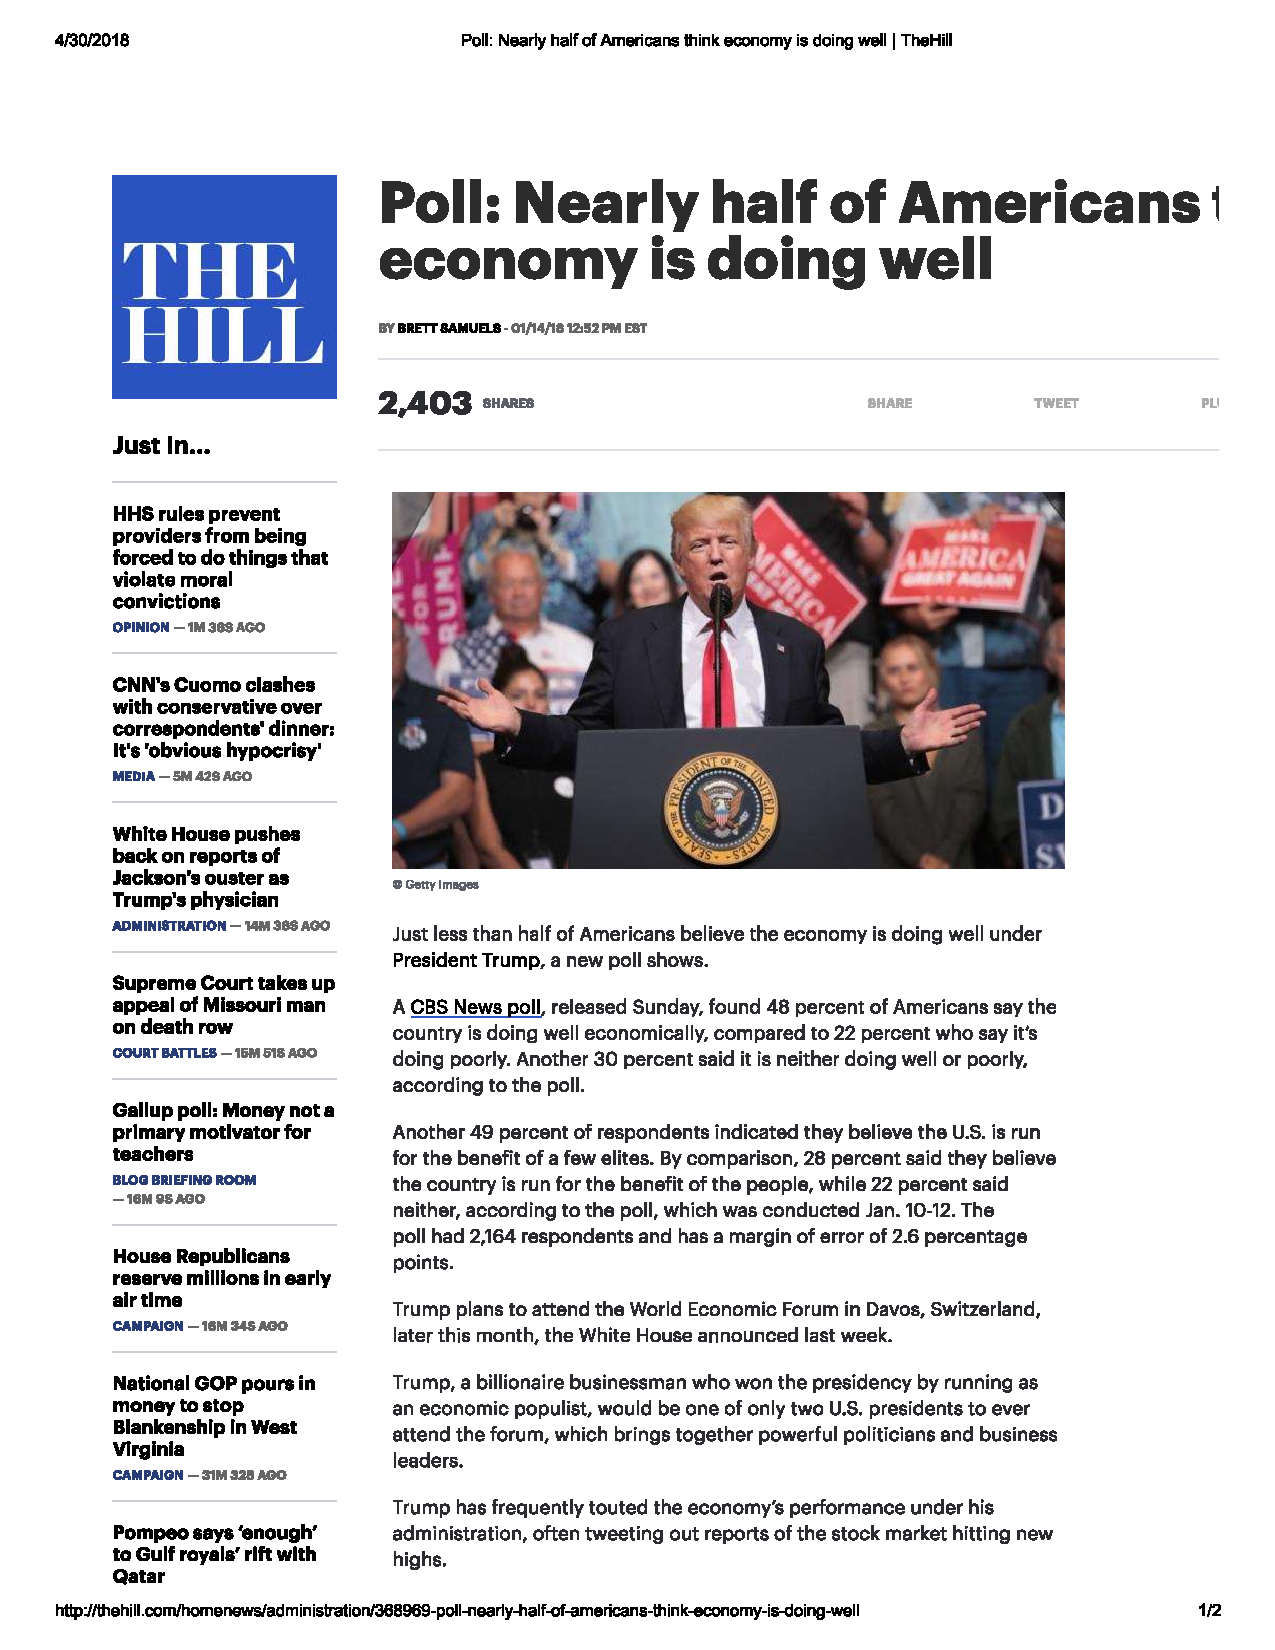
\includegraphics[width=1.05\textwidth]{control.pdf}
\smallskip
\end{figure}

\end{document}